\documentclass{beamer}

\mode<presentation>
{
  \usetheme{Madrid}
  \usecolortheme{default} 
  \usefonttheme{default}  
  \setbeamertemplate{navigation symbols}{}
  \setbeamertemplate{caption}[numbered]
  \setbeamertemplate{footline}[frame number] % Added from new slides
} 

\usepackage[english]{babel}
\usepackage[utf8]{inputenc}
\usepackage[T1]{fontenc}
\usepackage{amsmath}
\usepackage{amsfonts}
\usepackage{amssymb} 
\usepackage{booktabs}
\usepackage{array}
\usepackage{colortbl}
% left-aligned (ragged-right) fixed-width column: avoids stretched justification in tables
\newcolumntype{L}[1]{>{\raggedright\arraybackslash}p{#1}}
\usepackage{graphicx}
\usepackage{tikz}

% Merged TikZ libraries
\usetikzlibrary{positioning, calc, fit, arrows.meta, shapes.geometric, backgrounds, decorations.pathreplacing}

\graphicspath{{figures/}} 

% Color palette matching the diagrams
\definecolor{client}{RGB}{237,125,49}
\definecolor{server}{RGB}{68,114,196}
\definecolor{boxgray}{RGB}{240,240,240}
\definecolor{accent}{RGB}{112,48,160}

\title[NeuralPSI]{Privacy-Preserving Fingerprint Authentication}

\author[Pandey, Shil, Prusti]{
  Rineet Pandey, Ayan Shil, Prabhudutta Prusti \\[0.3cm]
  \small \textbf{Mentors:}\\
  Dr. Amit Kumar Chauhan, Ayan Chattopadhyay, \\Dr. Rohitkumar R. Upadhyay
}
\date{\today}

\begin{document}

\begin{frame}
  \titlepage
\end{frame}

\begin{frame}{Outline}
  \tableofcontents
\end{frame}

\section{Introduction}

\begin{frame}{What is a Fingerprint?}
  \begin{columns}[T]
    \begin{column}{0.55\textwidth}
      \begin{block}{Biological Identity}
        \begin{itemize}
          \item Ridges \& valleys form on the fingertip \emph{in utero} and never change.
          \item \textbf{Unique:} even identical twins differ.
          \item \textbf{Immutable:} the pattern persists for life.
          \item \textbf{Universal:} everyone has $\sim$10 fingers. 
          \item These properties make it ideal ID material - but also \alert{irreplaceable if leaked}.
        \end{itemize}
      \end{block}
      % Reduced from 0.3cm to 0.2cm to fix the 0.36pt overflow
      \vspace{0.2cm}
      \centering
      Identity $f: \text{finger} \to \text{pattern}$ 
      % Reduced from 2mm to 1mm
      \\[1mm]
      $\Pr[\text{same pattern, different finger}] \approx 0$
    \end{column}
    \begin{column}{0.45\textwidth}
      \centering
      \vspace*{0pt} 
      
      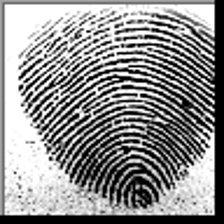
\includegraphics[width=0.55\linewidth]{alice_enrolled.png}
      \vspace{0.2cm}
      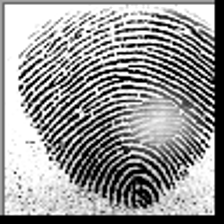
\includegraphics[width=0.55\linewidth]{alice_probe.png}
    \end{column}
  \end{columns}
\end{frame}

\begin{frame}{How Fingerprint Authentication Works}
  \begin{block}{The Standard Pipeline}
    \begin{enumerate}
      \item \textbf{Enroll:} capture the finger, extract features, store a \emph{template}.
      \item \textbf{Authenticate:} capture again, extract features, compare to stored template.
    \end{enumerate}
  \end{block}
  
  \vspace{0.2cm}
  \centering
  \resizebox{\textwidth}{!}{
  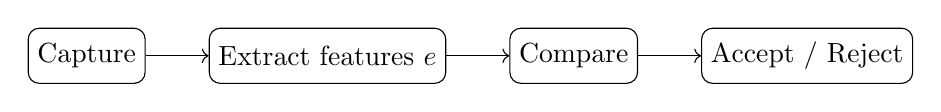
\begin{tikzpicture}[node distance=0.9cm, every node/.style={draw, rounded corners, minimum height=0.7cm}]
    \node (cap)  {Capture};
    \node (feat)[right=0.8cm of cap] {Extract features $e$};
    \node (comp)[right=0.8cm of feat] {Compare};
    \node (dec) [right=0.8cm of comp] {Accept / Reject};
    \draw[->] (cap) -- (feat);
    \draw[->] (feat) -- (comp);
    \draw[->] (comp) -- (dec);
  \end{tikzpicture}
  }
  \vspace{0.2cm}
  
  \[
    \text{score}(e_{\text{probe}}, e_{\text{gal}}) > \theta \;\Longrightarrow\; \text{genuine}
  \]
  
  \vspace{0.2cm}
  {\small\emph{Here "features" are the 16-D CNN embedding and "compare" is the fuzzy PSI match - done in private.}}
\end{frame}

\begin{frame}{The Problem}
  \begin{block}{Biometrics are the worst password}
    \begin{itemize}
      \item A password can be rotated. \textbf{A fingerprint cannot.}
      \item If a cryptographic key leaks - regenerate it. If a biometric leaks - \alert{forever compromised}.
    \end{itemize}
  \end{block}
  \begin{block}{The trusting-honest-third-party catch}
    \begin{itemize}
      \item Legacy methods authenticate via a private \emph{matching} service - the matcher sees every biometric.
      \item \textbf{We need to verify a fingerprint without anyone learning it} - or even learning whether a match happened.
    \end{itemize}
  \end{block}
  \[
    \underbrace{\text{verify}(x, Y)}_{\text{match-ness only}} \neq \underbrace{Y}_{\text{the database}}
  \]
\end{frame}

\begin{frame}{Current Cryptographic Tools \& Their Limits}
  \centering
  {\footnotesize Every prior family either \alert{cannot tolerate biometric noise},
  \alert{loses accuracy}, or \alert{pays a heavy cryptographic overhead}.}
  \vspace{0.15cm}

  \begin{table}
    \centering
    \scriptsize
    \setlength{\extrarowheight}{2pt}
    \begin{tabular}{@{}L{1.75cm}L{2.05cm}L{2.75cm}L{3.05cm}@{}}
      \toprule
      \textbf{Tool} & \textbf{Citation} & \textbf{Approach} & \textbf{Limitation} \\
      \midrule
      \rowcolor{gray!12}
      One-way hash & standard & Compare digests $f_k(x)$ & \textcolor{red}{Exact match only} \\
      Fuzzy commitment & Juels \& Wattenberg'99 & XOR with an ECC codeword & Needs ordered features; leaks \\
      \rowcolor{gray!12}
      Fuzzy vault & Juels \& Sudan'02 & Minutiae hidden in chaff & Correlation attacks; not revocable \\
      Fuzzy extractors & Dodis et al.'04 & Stable key $+$ helper data & High error rate; entropy loss \\
      \rowcolor{gray!12}
      Cancelable / BioHashing & Ratha'01; Teoh'04 & Non-invertible keyed transform & Accuracy drop; token secrecy \\
      HE (Blind-Touch) & Choi et al., AAAI'24 & CKKS-encrypted matching & 117\,MB key; $\sim$5k cap; score only \\
      \rowcolor{gray!22}
      \textbf{FLPSI} & Uzun'21; Bui \& Cong'25 & mOPRF $+$ threshold PSI & \textbf{Needs binary Hamming codes} \\
      \bottomrule
    \end{tabular}
  \end{table}
\end{frame}

\begin{frame}{The Closest Prior Work: Blind-Touch (AAAI 2024)}
  \begin{block}{What it does}
    \begin{itemize}
      \item A Siamese CNN maps a fingerprint to a \textbf{16-D embedding}; matching runs under CKKS homomorphic encryption, so the server never decrypts:
      $\textsf{Dec}\big(\textsf{Eval}(f,\textsf{Enc}(x))\big) = f(x)$.
      \item \textbf{We reuse its feature extractor} - the accuracy comes from the CNN, not the encryption.
    \end{itemize}
  \end{block}

  \begin{block}{Its three limitations - and our opening}
    \begin{itemize}
      \item \textbf{Huge keys:} a 117\,MB Galois rotation key on every server.
      \item \textbf{Scale ceiling:} $8{,}192$ slots $\div\,16 = 512$ users per ciphertext; impractical beyond \alert{$\sim$5{,}000 users}.
      \item \textbf{No labels:} returns a match \emph{score} only - never \emph{which} record matched.
    \end{itemize}
  \end{block}
  \centering
  \emph{The matching layer is the bottleneck - so we replace it.}
\end{frame}

\begin{frame}
  \centering
  \vspace{2cm}
  {\Huge \textbf{Our Proposed Solution:}} \\[0.6em]
  {\Huge \textbf{\alert{Neural PSI}}}
\end{frame}

\begin{frame}{What is Private Set Intersection (PSI)?}
  \begin{block}{Formal Definition}
    \begin{itemize}
      \item Two parties, sets $X$ (Alice) and $Y$ (Bob).
      \item They learn only the intersection $X \cap Y$ - and nothing else.
    \end{itemize}
  \end{block}
  
  \[
    \text{PSI}(X,Y) \to X \cap Y, \quad \text{leakage } \mathcal{L}=X\cap Y \text{ only}
  \]
  
  \begin{block}{Why PSI for biometrics?}
    \begin{itemize}
      \item Naive match: compare $e$ to every $y \in Y$ - leaks mass information.
      \item \textbf{Asymmetric matching:} Alice learns the \emph{label of her match}, Bob learns \emph{nothing}.
      \item \textbf{But} biometric codes are \emph{noisy} - exact set membership fails.
      \item $\Rightarrow$ \alert{Fuzzy} / threshold PSI (FLPSI) tolerates $t$ out of $T$ sub-matches.
    \end{itemize}
  \end{block}
\end{frame}



\section{System Architecture \& Feature Extraction}

\begin{frame}{System Architecture}
  \vspace{-0.3ex}
  \centering
  \makebox[\textwidth][c]{%
    \includegraphics[width=1.05\textwidth,
                     trim=8 8 8 8, clip]%
      {neuralpsi-architecture.png}}
  \vfill
\end{frame}

% \begin{frame}{System Architecture}
%   \centering
%   \resizebox{0.95\textwidth}{!}{
%   \begin{tikzpicture}[
%       clientbox/.style={draw=blue!70, fill=white, thick, rounded corners=4pt, align=center, minimum width=5.0cm, minimum height=0.8cm},
%       serverbox/.style={draw=teal!70, fill=white, thick, rounded corners=4pt, align=center, minimum width=5.0cm, minimum height=0.8cm},
%       arrow/.style={-stealth, thick, draw=gray!80!black},
%       darrow/.style={stealth-stealth, thick, dashed, draw=gray!80!black}
%     ]
    
%     \node[draw=blue!30, fill=blue!5, rounded corners=8pt, thick, minimum width=5.8cm, minimum height=7.2cm] (clientbg) at (0, -3.2) {};
%     \node[font=\normalsize\bfseries\color{blue!80!black}, anchor=north, yshift=-0.2cm] at (clientbg.north) {CLIENT DEVICE \small(plaintext)};
    
%     \node[draw=teal!30, fill=teal!5, rounded corners=8pt, thick, minimum width=5.8cm, minimum height=7.2cm] (serverbg) at (9.0, -3.2) {};
%     \node[font=\normalsize\bfseries\color{teal!80!black}, anchor=north, yshift=-0.2cm] at (serverbg.north) {SERVER \small(cryptographic)};
    
%     \node[clientbox] (c1) at (0, -1.0) {Fingerprint Image};
%     \node[clientbox] (c2) at (0, -2.2) {Siamese CNN Feature Extr. \\[-0.5ex] {\scriptsize (5 Conv Blocks $\to$ FC-16)}};
%     \node[clientbox] (c3) at (0, -3.4) {16-D Float Embedding $e$ \\[-0.5ex] {\scriptsize (unit-normalized)}};
%     \node[clientbox] (c4) at (0, -4.6) {Super-Bit Quantizer \\[-0.5ex] {\scriptsize (center $\to$ project $\to$ sign)}};
%     \node[clientbox] (c5) at (0, -5.8) {128-bit Binary Code $b$};
    
%     \node[serverbox, minimum height=2.2cm] (s1) at (9.0, -2.8) {\textbf{FLPSI Protocol Engine} \\[1.5ex] mOPRF (GC) \\ TLPSI (VOLE) \\ Shamir Recovery};
%     \node[serverbox] (s2) at (9.0, -5.8) {\textbf{Template DB} \\[-0.5ex] {\scriptsize (128-bit codes + labels)} \\[-0.5ex] {\scriptsize 16 bytes/user}};
    
%     \draw[arrow] (c1) -- (c2);
%     \draw[arrow] (c2) -- (c3);
%     \draw[arrow] (c3) -- (c4);
%     \draw[arrow] (c4) -- (c5);
%     \draw[arrow] (s1) -- (s2);
    
%     \draw[darrow] (clientbg.east |- c3.south) -- 
%         node[above, align=center, font=\scriptsize\bfseries, text=black!80] {multi-round \\[-0.5ex] protocol} 
%         node[below, font=\scriptsize, text=black!80] {(per authentication)} 
%         (serverbg.west |- c3.south);
        
%     \draw[-stealth, thick, dashed, draw=gray!80!black] (serverbg.west |- c3.south) -- (s1.south west);
        
%     \draw[arrow] (c5.east) -- 
%         node[above, font=\scriptsize\bfseries, text=black!80] {register} 
%         node[below, font=\scriptsize, text=black!80] {(once per user)} 
%         (s2.west);
        
%   \end{tikzpicture}
%   }
% \end{frame}

\begin{frame}{Preprocessing \& Convolution}
  \begin{block}{Raw Input \& Preprocessing}
    \begin{itemize}
      \item $224\times224$ grayscale image normalized to $[0.0, 1.0]$.
      \item No alignment, filtering, or minutiae extraction.
      \item Augmented with rotation ($\pm15^\circ$), translation ($\pm6\%$), and Gaussian noise ($\sigma=6$).
    \end{itemize}
  \end{block}

  \begin{block}{Five Convolutional Blocks}
    \begin{itemize}
      \item $\text{Conv}(3\times3) \to \text{BatchNorm} \to \text{SiLU} \to \text{MaxPool}(2\times2)$.
      \item Channels grow $32\to64\to128\to256\to512$ while the map halves each block: $224\to112\to56\to28\to14\to7$.
      \item Progresses from detecting edges ($32\times112\times112$) to an abstract identity code ($512\times7\times7$).
    \end{itemize}
  \end{block}
\end{frame}

\begin{frame}{Feature Vector \& Siamese Training}
  \begin{block}{The FC-16 Output}
    \begin{itemize}
      \item Flattens the final spatial block ($512\times7\times7$) into \textbf{25,088} numbers.
      \item One linear layer $W \in \mathbb{R}^{25088\times16}$ produces the 16-D embedding $e \in \mathbb{R}^{16}$.
      \item \textbf{Client-side only:} The server never receives these continuous values.
    \end{itemize}
  \end{block}
  
  \vspace{0.3cm}
  \textbf{Siamese Loss Function:}
  \[
   L = -\mathbb{E}\big[\,y\log\sigma(w\cdot d(e_1,e_2)) + (1-y)\log\big(1-\sigma(w\cdot d(e_1,e_2))\big)\big]
  \]
\end{frame}

\section{Quantization}

\begin{frame}{Why Super-Bit? Binarization Method Comparison}
  \centering
  {\footnotesize Three binarization schemes evaluated on SOCOFing - only Super-Bit achieves
  \emph{both} similarity preservation and $50/50$ bit balance.}
  \vspace{0.1cm}

  \begin{table}
    \centering
    \scriptsize
    \setlength{\extrarowheight}{2pt}
    \begin{tabular}{@{}l L{2.6cm} L{2.6cm} L{3.0cm}@{}}
      \toprule
       & \textbf{Method 1: sign$(>0)$} & \textbf{Method 2: ITQ} & \textbf{Method 3: Super-Bit $\star$} \\
      \midrule
      \textbf{Bits} & 16 & 16 & \textbf{128} \\
      \textbf{Rule} & $b_k=\mathbf{1}[e_k>0]$ & $b=\mathrm{sign}\big((e-\mu)R\big)$ & $b=\mathbf{1}[P e_0 > \tau]$ \\
      \midrule
      \rowcolor{gray!12}
      \textbf{Idea}
        & Threshold each float at zero
        & Learn rotation $R$ to align axes
        & Expand 16 floats $\to$ 128 bits \\
      \rowcolor{gray!12}
      \textbf{Issue}
        & Borderline bits flip; only $2^{16}$ codes
        & Fixes flips, but still 16 bits
        & 8 orthonormal blocks; median $\tau$ gives $50/50$ \\
      \midrule
      \textbf{EER} $96^2$   & 10.86\% & 7.12\% & 5.14\% \\
      \textbf{EER} $224^2$  & 10.12\% & 5.55\% & \textbf{1.88\%} \\
      \midrule
      \textbf{Verdict} & \textcolor{red}{Rejected} & \textcolor{red}{Rejected} & \textbf{\checkmark\ Chosen} \\
      \bottomrule
    \end{tabular}
  \end{table}
  {\scriptsize Only Super-Bit has enough code space \emph{and} a minimum-variance angular estimate.}
\end{frame}

\begin{frame}{The Three Quantization Stages}
  \begin{block}{Stage 1 - Population Centering \hfill $e_0 = e - \mu$}
    {\footnotesize Embeddings cluster in a few directions, so origin hyperplanes give
    \alert{unbalanced bits}. Subtract the population mean $\mu$ (computed offline).}
  \end{block}

  \begin{block}{Stage 2 - Super-Bit Projection \hfill $z = P e_0,\; P^\top=[Q_1,\dots,Q_8]$}
    {\footnotesize Random projections are redundant. Each block is Gaussian, then Gram--Schmidt
    orthonormalized ($Q_j^\top Q_j = I_{16}$), giving a \textbf{minimum-variance} angular estimate.}
  \end{block}

  \begin{block}{Stage 3 - Balanced Median Thresholding \hfill $b_k = \mathbf{1}[z_k > \tau_k]$}
    {\footnotesize FLPSI requires \textbf{maximum entropy per bit} ($50/50$). The public median
    threshold $\tau$ guarantees it.}
  \end{block}

  \vspace{0.15cm}
  {\footnotesize \textbf{Evaluated and rejected - metric whitening.} An optional
  $e_1=\mathrm{diag}\big(\sqrt{|w_1|}\big)e_0$ step rescales axes by the head's learned weights.
  It helps a \emph{weak} model ($5.14\%\!\to\!3.91\%$) but \alert{hurts the trained one}
  ($1.88\%\!\to\!2.98\%$), so the deployed pipeline omits it.}
\end{frame}

\begin{frame}{Chosen Method: Super-Bit LSH}
  \begin{block}{Super-Bit Projection \& Thresholding}
    \begin{itemize}
      \item Expands 16 floats into 128 bits using 8 orthonormal Gram-Schmidt blocks.
      \item Median $\tau$ guarantees a $50/50$ balance, and it provides a minimum-variance angular estimate.
    \end{itemize}
  \end{block}
  
  \vspace{0.2cm}
  \textbf{Projection Matrices \& Binarization:}
  \[
    P^\top = [Q_1,\dots,Q_8] \text{ with } Q_j^\top Q_j = I_{16}
  \]
  \[
    b_k = \mathbf{1}[z_k > \tau_k]
  \]
\end{frame}

\section{Cryptography: The FLPSI Engine}

\begin{frame}{The Problem: }
  \begin{columns}[T, onlytextwidth]
    \begin{column}{0.48\textwidth}
      \textbf{Two templates. Never exactly equal.}
      \vspace{4pt}
      
      Two scans of the \emph{same} finger almost never produce identical
      binary codes - noise, rotation, and pressure all shift a few bits.
      
      \vspace{8pt}
      \begin{block}{\small What we actually need}
      \centering
      \small
      $d_H(x, y_i) \le d_k \;\Rightarrow\; \text{reveal } \ell_i$
      \end{block}
      
      \vspace{6pt}
      \small Ordinary PSI only tests \emph{exact} equality ($x = y_i$).
      It has no notion of ``close enough.''
    \end{column}
    \hfill
    \begin{column}{0.48\textwidth}
      \begin{block}{\small Enter FLPSI}
      \small
      \textbf{Fuzzy Labelled Private Set Intersection} tolerates bounded
      Hamming error under a precise leakage profile $\mathcal{L}$:
      \begin{itemize}
        \small
        \item Server learns \textbf{nothing}.
        \item Client learns the \textbf{label} on a match, \emph{plus} which
        sub-samples collided - never the stored template itself.
      \end{itemize}
      \end{block}
      \vspace{6pt}
      
    \end{column}
  \end{columns}
\end{frame}

\begin{frame}{Cryptography Stack}
  \centering
  \resizebox{0.95\textwidth}{!}{
  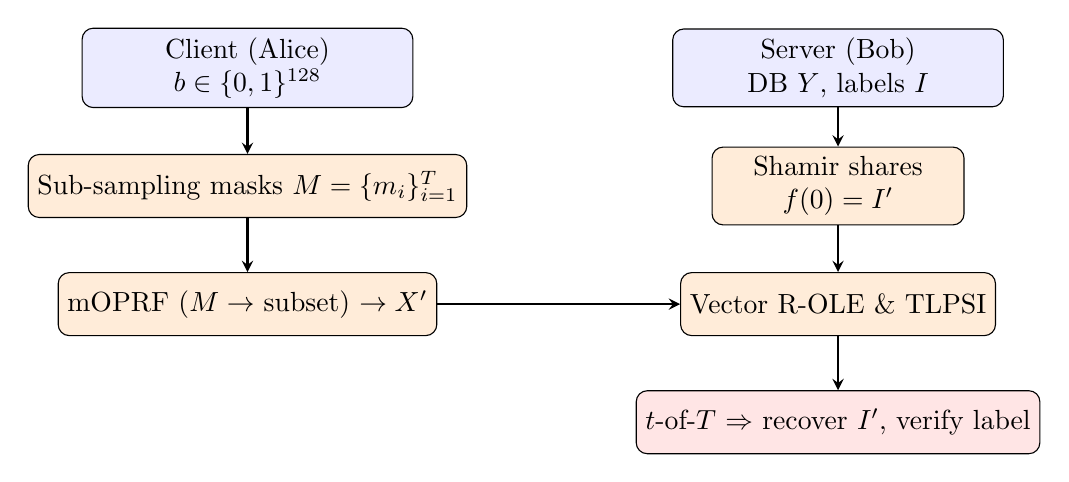
\begin{tikzpicture}[
      box/.style={draw, rounded corners, fill=blue!8, minimum width=4.2cm, minimum height=0.9cm, align=center},
      crypto/.style={draw, rounded corners, fill=orange!15, minimum width=3.2cm, minimum height=0.8cm, align=center},
      arrow/.style={-stealth, thick}
    ]
    
    % Client column (Left)
    \node[box] (client) at (0,7) {Client (Alice) \\ $b \in \{0,1\}^{128}$};
    \node[crypto] (masks) at (0,5.5) {Sub-sampling masks $M=\{m_i\}_{i=1}^{T}$};
    \node[crypto] (oprf)  at (0,4) {mOPRF ($M \to$ subset) $\to X'$};
    
    % Server column (Right)
    \node[box] (server) at (7.5,7) {Server (Bob) \\ DB $Y$, labels $I$};
    \node[crypto] (shamir) at (7.5,5.5) {Shamir shares \\ $f(0)=I'$};
    \node[crypto] (vrole)  at (7.5,4) {Vector R-OLE \& TLPSI};
    
    % Output (Directly below Server column)
    \node[crypto, fill=red!10] (out) at (7.5,2.5) {$t$-of-$T$ $\Rightarrow$ recover $I'$, verify label};
    
    % Core Flow 
    \draw[arrow] (client.south) -- (masks.north);
    \draw[arrow] (masks.south) -- (oprf.north);
    \draw[arrow] (server.south) -- (shamir.north);
    \draw[arrow] (shamir.south) -- (vrole.north);
    \draw[arrow] (vrole.south) -- (out.north);
    
    % Cross-party Flow 
    \draw[arrow] (oprf.east) -- (vrole.west);
    
  \end{tikzpicture}
  }
  \vspace{0.4cm}

\end{frame}

\begin{frame}{Primitive 1: Masked Oblivious PRF (mOPRF)}
  \textbf{The problem:} sub-sampling $x \wedge m_j$ directly would leak
  biometric bits whenever a match occurs.
  
  \vspace{10pt}
  \begin{center}
  \resizebox{0.95\textwidth}{!}{
  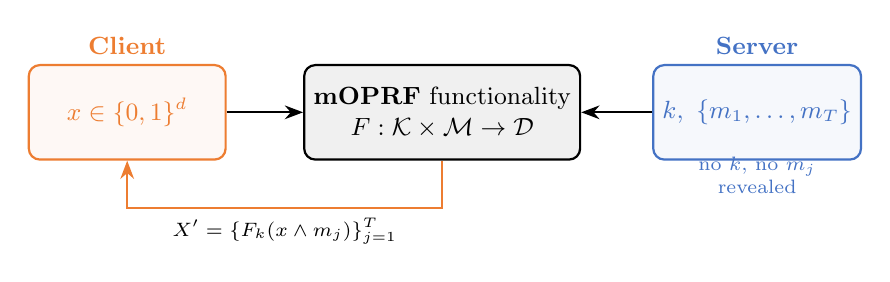
\begin{tikzpicture}[>=Stealth, font=\small, node distance=5mm]
    % Client Box
    \node[draw, thick, color=client, fill=client!5, rounded corners, minimum width=2.5cm, minimum height=1.2cm, align=center, label={[color=client]above:\textbf{Client}}] (C) at (0,0) {$x\in\{0,1\}^d$};
    
    % Server Box
    \node[draw, thick, color=server, fill=server!5, rounded corners, minimum width=2.5cm, minimum height=1.2cm, align=center, label={[color=server]above:\textbf{Server}}] (S) at (8,0) {$k,\ \{m_1,\dots,m_T\}$};
    
    % mOPRF Box
    \node[draw, thick, rounded corners, fill=boxgray, minimum width=3.4cm, minimum height=1.2cm, align=center] (F) at (4,0) {\textbf{mOPRF} functionality\\ $F: \mathcal{K}\times\mathcal{M}\to\mathcal{D}$};
    
    \draw[->, thick] (C) -- (F);
    \draw[->, thick] (S) -- (F);
    
    \draw[->, thick, color=client] (F.south) -- +(0,-0.6) -| (C.south) 
      node[pos=0.25, below, font=\scriptsize, text=black]{$X' = \{F_k(x\wedge m_j)\}_{j=1}^T$};
    
    \node[align=center,font=\scriptsize, color=server] at (8,-0.8) {no $k$, no $m_j$\\revealed};
  \end{tikzpicture}
  }
  \end{center}
  \vspace{6pt}
  
  \begin{block}{\small Why it works}
  \small
  \[
  F_k(x\wedge m_j) = F_k(y\wedge m_j) \iff x\wedge m_j = y \wedge m_j
  \]
  \end{block}
  \small Equality of sub-samples is preserved; the sub-samples themselves
  are computationally hidden - deterministic \emph{and} pseudorandom.
\end{frame}

\begin{frame}{Primitive 2: Vector Oblivious Linear Evaluation (VOLE)}
  \textbf{The problem:} generating $n$ independent correlations via $n$
  \textbf{Oblivious Linear Evaluation (OLE)} calls is far too slow for millions of matches.
  
  \vspace{10pt}
  \begin{center}
  \resizebox{0.95\textwidth}{!}{
  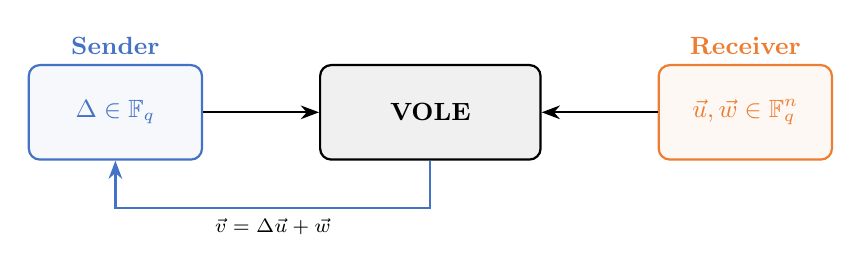
\begin{tikzpicture}[>=Stealth, font=\small]
    % Sender Box
    \node[draw, thick, color=server, fill=server!5, rounded corners, minimum width=2.2cm, minimum height=1.2cm, align=center, label={[color=server]above:\textbf{Sender}}] (S) at (0,0) {$\Delta \in \mathbb{F}_q$};
    
    % Receiver Box
    \node[draw, thick, color=client, fill=client!5, rounded corners, minimum width=2.2cm, minimum height=1.2cm, align=center, label={[color=client]above:\textbf{Receiver}}] (C) at (8,0) {$\vec u,\vec w \in \mathbb{F}_q^n$};
    
    % VOLE Box
    \node[draw, thick, rounded corners, fill=boxgray, minimum width=2.8cm, minimum height=1.2cm] (V) at (4,0) {\textbf{VOLE}};
    
    \draw[->, thick] (S) -- (V);
    \draw[->, thick] (C) -- (V);
    \draw[->, thick, color=server] (V.south) -- +(0,-0.6) -| (S.south)  
      node[pos=0.25, below, font=\scriptsize, text=black]{$\vec v = \Delta\vec u+\vec w$};
  \end{tikzpicture}
  }
  \end{center}
  \vspace{6pt}
  
  \begin{block}{\small The linear correlation}
  \[
  v_i = u_i \Delta + w_i,\qquad 1\le i \le n \qquad\Longleftrightarrow\qquad \vec v = \Delta \vec u + \vec w
  \]
  \end{block}
  \small
  \textbf{Sender} knows $(\Delta,\vec v)$; \textbf{receiver} knows $(\vec u,\vec w)$
  - neither alone can reconstruct the relation, yet together it holds
  exactly. This one relation is the seed for everything that follows.
\end{frame}

\begin{frame}{Silent VOLE Extension: From a Few to Millions}
  \textbf{The problem:} FLPSI needs \emph{millions} of VOLE correlations
  per query - one base VOLE per correlation is impossibly expensive.
  
  \vspace{10pt}
  \begin{center}
  \resizebox{\textwidth}{!}{
  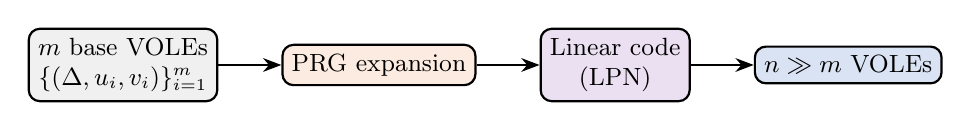
\begin{tikzpicture}[>=Stealth, font=\small, node distance=8mm]
    \node[draw, thick, rounded corners, fill=boxgray, align=center] (base) {$m$ base VOLEs\\ $\{(\Delta,u_i,v_i)\}_{i=1}^m$};
    \node[draw, thick, rounded corners, fill=client!15, right=of base] (prg) {PRG expansion};
    \node[draw, thick, rounded corners, fill=accent!15, right=of prg, align=center] (lpn) {Linear code\\ (LPN)};
    \node[draw, thick, rounded corners, fill=server!20, right=of lpn] (many) {$n \gg m$ VOLEs};
    \draw[->, thick] (base) -- (prg);
    \draw[->, thick] (prg) -- (lpn);
    \draw[->, thick] (lpn) -- (many);
  \end{tikzpicture}
  }
  \end{center}
  
  \vspace{10pt}
  \begin{block}{\small Why LPN?}
  \small \begin{itemize}
    \item Expands a few VOLEs into millions.
    \item Preserves VOLE correlations.
    \item Computationally indistinguishable from random.
\end{itemize}
  \end{block}
\end{frame}

\begin{frame}{Primitive 3: Vector Ring-VOLE - VOLE Meets Polynomials}
  \textbf{The problem:} TLPSI needs \emph{polynomial products}, not just
  scalar correlations - Vector-VOLE alone cannot multiply polynomials.
  
  \vspace{2pt}
  \begin{block}{\small Setup (evaluation-point trick)}
  \footnotesize
  Receiver holds $u_0(x)$, $\deg \le d$; sender holds $\{v_i(x)\}_{i=1}^m$,
  $\deg \le 2d$. Both evaluate over a public set $X=\{x_1,\dots,x_{2d+1}\}$:
  \[
  U_i = u_i(X), \quad V_i = v_i(X), \quad Z_i = u_0(X)\odot U_i + V_i
  \]
  \end{block}
  \vspace{-2pt}
  \begin{center}
  \resizebox{0.85\textwidth}{!}{
  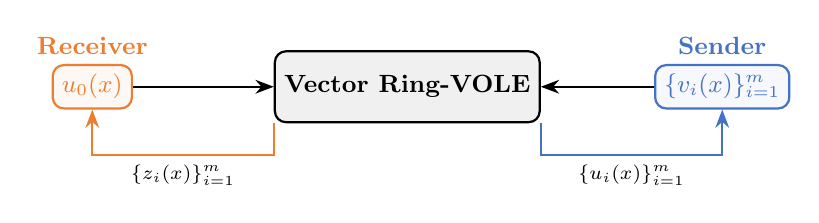
\begin{tikzpicture}[>=Stealth,font=\small]
    % Receiver
    \node[draw, thick, color=client, fill=client!5, rounded corners, align=center, label={[color=client]above:\textbf{Receiver}}] (C) at (0,0) {$u_0(x)$};
    % Sender
    \node[draw, thick, color=server, fill=server!5, rounded corners, align=center, label={[color=server]above:\textbf{Sender}}] (S) at (8,0) {$\{v_i(x)\}_{i=1}^m$};
    
    % Ring-VOLE
    \node[draw, thick, rounded corners, fill=boxgray, minimum width=3.2cm, minimum height=0.9cm] (R) at (4,0) {\textbf{Vector Ring-VOLE}};
    
    \draw[->, thick] (C) -- (R);
    \draw[->, thick] (S) -- (R);
    
    \draw[->, thick, color=client] (R.south west) -- +(0,-0.4) -| (C.south) 
      node[pos=0.25, below, text=black, font=\scriptsize] {$\{z_i(x)\}_{i=1}^m$};
    \draw[->, thick, color=server] (R.south east) -- +(0,-0.4) -| (S.south) 
      node[pos=0.25, below, text=black, font=\scriptsize] {$\{u_i(x)\}_{i=1}^m$};
  \end{tikzpicture}
  }
  \end{center}
  \vspace{-2pt}
  
\end{frame}



\begin{frame}{From Ring-VOLE to Threshold Labelled PSI (TLPSI)}
  \textbf{The idea:} represent a \emph{set} by the polynomial whose roots
  are its elements.
  
  \vspace{2pt}
  \begin{center}
  \resizebox{0.85\textwidth}{!}{
  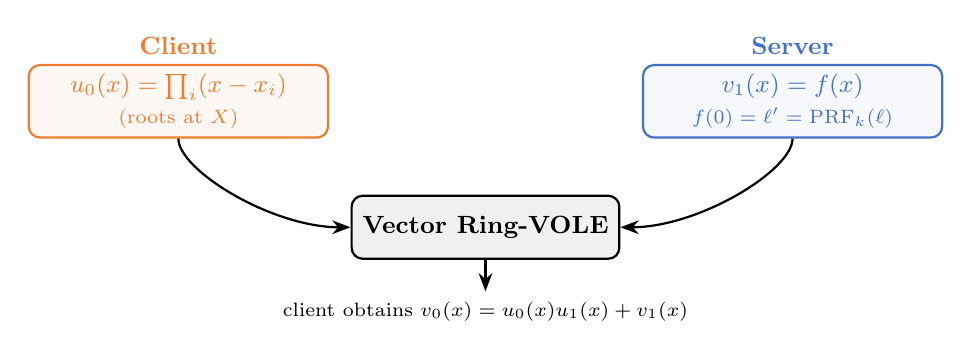
\begin{tikzpicture}[>=Stealth,font=\small]
    \node[draw, thick, color=client, fill=client!5, rounded corners, align=center, minimum width=3.8cm, label={[color=client]above:\textbf{Client}}] (C) at (0,1.0) {$u_0(x)=\prod_{i}(x-x_i)$\\ \scriptsize (roots at $X$)};
    
    \node[draw, thick, color=server, fill=server!5, rounded corners, align=center, minimum width=3.8cm, label={[color=server]above:\textbf{Server}}] (S) at (7.8,1.0) {$v_1(x)=f(x)$\\ \scriptsize $f(0)=\ell'=\mathrm{PRF}_k(\ell)$};
    
    \node[draw, thick, rounded corners, fill=boxgray, minimum width=3.4cm, minimum height=0.8cm] (RV) at (3.9,-0.6) {\textbf{Vector Ring-VOLE}};
    
    \draw[->, thick] (C.south) .. controls +(0,-0.4) and +(-1,0) .. (RV.west);
    \draw[->, thick] (S.south) .. controls +(0,-0.4) and +(1,0) .. (RV.east);
    \draw[->, thick] (RV.south) -- +(0,-0.4) node[below,font=\scriptsize,align=center] {client obtains $v_0(x)=u_0(x)u_1(x)+v_1(x)$};
  \end{tikzpicture}
  }
  \end{center}
  \vspace{2pt}
  
  \begin{block}{\small The magic identity}
  \footnotesize For $x_i \in X\cap Y$: $u_0(x_i)=0 \Rightarrow v_0(x_i)=v_1(x_i)=f(x_i)$.
  \end{block}
  \vspace{-2pt}
  \footnotesize Every common element yields one true evaluation of the Shamir
  polynomial $f$. Collect $\ge t$ of them $\Rightarrow$ interpolate
  $f(0)=\ell'$; reveal $\ell$ after checking validity. Fewer than $t \Rightarrow$ information-theoretically hidden.
\end{frame}

\begin{frame}{The Full FLPSI Protocol: mOPRF $+$ TLPSI}
  \centering
  \resizebox{\textwidth}{!}{
  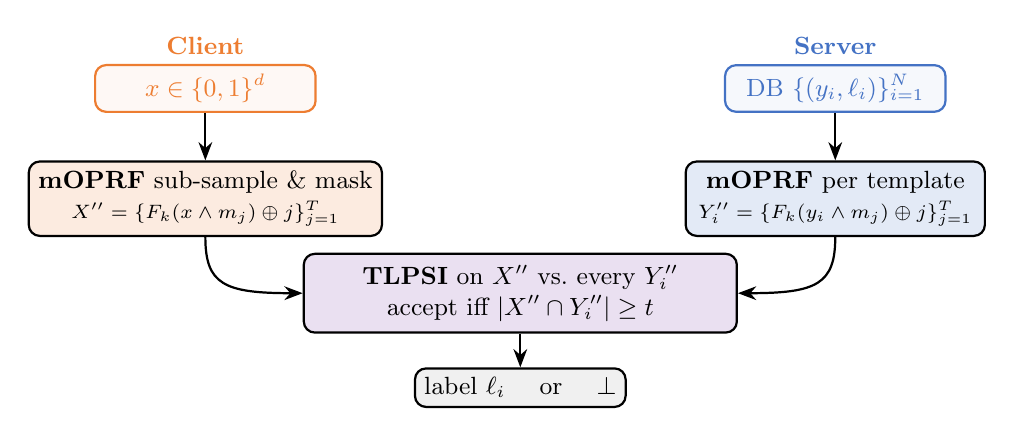
\begin{tikzpicture}[>=Stealth, font=\small, node distance=5mm]
  
    \node[draw, thick, color=client, fill=client!5, rounded corners, align=center, minimum width=2.8cm, label={[color=client]above:\textbf{Client}}] (x) at (1.5,2.6) {$x\in\{0,1\}^{d}$};
    
    \node[draw, thick, color=server, fill=server!5, rounded corners, align=center, minimum width=2.8cm, label={[color=server]above:\textbf{Server}}] (Y) at (9.5,2.6) {DB $\{(y_i,\ell_i)\}_{i=1}^N$};
    
    \node[draw, thick, rounded corners, fill=client!15, minimum width=3.8cm, align=center] (mo) at (1.5,1.2)
      {\textbf{mOPRF} sub-sample \& mask\\ \scriptsize $X''=\{F_k(x\wedge m_j)\oplus j\}_{j=1}^{T}$};
    
    \node[draw, thick, rounded corners, fill=server!15, minimum width=3.8cm, align=center] (moY) at (9.5,1.2)
      {\textbf{mOPRF} per template\\ \scriptsize $Y_i''=\{F_k(y_i\wedge m_j)\oplus j\}_{j=1}^{T}$};
    
    \draw[->, thick] (x) -- (mo);
    \draw[->, thick] (Y) -- (moY);
    
    \node[draw, thick, rounded corners, fill=accent!15, minimum width=5.5cm, minimum height=1cm, align=center]
      (tl) at (5.5,0) {\textbf{TLPSI} on $X''$ vs.\ every $Y_i''$\\ accept iff $|X''\cap Y_i''|\ge t$};
    
    \draw[->, thick] (mo.south) .. controls +(0,-0.6) and +(-1,0) .. (tl.west);
    \draw[->, thick] (moY.south) .. controls +(0,-0.6) and +(1,0) .. (tl.east);
    
    \node[draw, thick, rounded corners, fill=boxgray, align=center] (out) at (5.5,-1.2) {label $\ell_i$ \quad or \quad $\bot$};
    \draw[->, thick] (tl) -- (out);
  
  \end{tikzpicture}
  }
  
  \vspace{12pt}
  \begin{block}{\small Intuition: Closeness Translates to Threshold Intersection}
  \small If the Hamming distance between the templates is small, enough sub-samples will naturally collide to hit our intersection threshold $t$. 
  \end{block}
\end{frame}

\begin{frame}{Security Analysis}
  \begin{block}{\small Theorem (informal)}
  \small NeuralPSI securely realizes FLPSI in the
  $\{\mathcal{F}^{T,t}_{\text{TLPSI}}, \mathcal{F}^T_{\text{mOPRF}}\}$-hybrid
  model against semi-honest adversaries.
  \end{block}
  
  \vspace{8pt}
  \small
  \begin{enumerate}
    \item CNN runs strictly locally - no raw biometric ever leaves the client.
    \item Server only ever sees \textbf{PRF-masked sub-samples} of $\tilde x$,
    never $\tilde x$ itself.
    \item The core FLPSI argument composes securely via a standard
    hybrid argument.
  \end{enumerate}
\end{frame}



\section{Performance Evaluation}

\begin{frame}
  \centering
  \vspace{2.4cm}
  {\Huge \textbf{\alert{Demonstration}}}
\end{frame}

\begin{frame}{Final Results \& Accuracy}
  \begin{block}{Accuracy \& Storage Milestones}
    \begin{itemize}
      \item Retains 1.88\% EER, comparable to continuous float accuracy ceilings.
      \item Achieves a 107x reduction in per-user template size (down to 16 Bytes).
    \end{itemize}
  \end{block}

  \begin{table}
    \centering
    \caption{Open-set EER on SOCOFing ($224\times224$ CNN model)}
    \begin{tabular}{lcc}
      \toprule
      \textbf{Representation} & \textbf{Bits} & \textbf{EER} \\ 
      \midrule
      Float features (HE ceiling) & - & 0.33\% \\
      $\text{sign}(>0)$ & 16 & 10.12\% \\
      ITQ & 16 & 5.55\% \\
      \textbf{Super-Bit (recommended)} & \textbf{128} & \textbf{1.88\%} \\
      + metric whitening & 128 & 2.98\% \\ 
      \bottomrule
    \end{tabular}
  \end{table}
\end{frame}

\begin{frame}{Latency, Storage \& Communication}
  \begin{table}
    \centering
    \scriptsize
    \setlength{\extrarowheight}{1.8pt}
    \begin{tabular}{@{}L{3.9cm}L{3.0cm}L{3.0cm}@{}}
      \toprule
      & \textbf{Blind-Touch (HE/CKKS)} & \textbf{NeuralPSI (ours)} \\
      \midrule
      \rowcolor{gray!12}
      \textbf{Servers used} & 1 main $+$ 3 cluster & \textbf{1} \\
      \textbf{Latency, single server} & 1{,}334\,ms & \textbf{$\sim$824\,ms} \\
      \midrule
      \textbf{Template per user} & 1.67\,KB & \textbf{16\,B} \\
      \rowcolor{gray!12}
      \textbf{Evaluation (Galois) key} & 117\,MB & \textbf{none} \\
      \midrule
      \textbf{Per-query data} ($N=5{,}000$) & 856\,KB ciphertext & 7.77\,MB \\
      \rowcolor{gray!12}
      \quad per record & - & 1.54\,KB \\
      \quad at $10^5$ / $10^6$ & - & $\sim$150\,MB / $\sim$1.5\,GB \\
      \midrule
      \rowcolor{gray!12}
      \textbf{Capacity} & 512 users/ciphertext & linear in $N$ \\
      \bottomrule
    \end{tabular}
  \end{table}

  \vspace{0.35cm}
  {\scriptsize
  Blind-Touch: Choi, Woo \& Kim, AAAI 2024 (Tables 2 and 8). NeuralPSI measured single-host on the
  real protocol binary: 0.80\,ms CNN $+$ 823\,ms matching; $10^5/10^6$ extrapolated from
  $\approx0.25$\,MB $+\,1.54$\,KB$\cdot N$, against Bui \& Cong's reported 153\,MB / 1533\,MB.}
\end{frame}

\begin{frame}{Conclusion \& Future Work}
  \begin{block}{Conclusion}
    {\footnotesize
    \begin{itemize}\itemsep2pt
      \item Fingerprint authentication \textbf{without revealing the biometric}, no trusted third party.
      \item The \textbf{binarization bridge} makes a CNN and Fuzzy Labelled PSI compatible.
      \item HE $\to$ VOLE $+$ Shamir: \textbf{16\,B/user} ($\sim$107$\times$ smaller), \textbf{no 117\,MB key}; \textbf{sub-second at $N=5{,}000$}, and linear $+$ shardable past $10^6$.
    \end{itemize}}
  \end{block}

  \begin{block}{Future Work}
    {\footnotesize
    \begin{itemize}\itemsep2pt
      \item \textbf{Larger datasets:} cross-sensor / cross-session (e.g.\ PolyU) - the real credibility test.
      \item \textbf{Algorithm:} accuracy saturates at 128 bits, so the \alert{16-D embedding} is the bottleneck - widen it; extend to malicious security.
      \item \textbf{Parallel processing:} the FLPSI scan is linear and embarrassingly parallel - shard it, precompute the offline phase.
      \item \textbf{Research paper:} formal security proof $+$ integrated prototype.
    \end{itemize}}
  \end{block}
\end{frame}

\begin{frame}
  \centering
  \vspace{2cm}
  {\Huge \textbf{Thank You}} \\[1em]
  {\Large Questions?}
\end{frame}

\end{document}